% \begin{document}
\chapter{Programmazione Lineare}
\section{Geometria della PL}
Ci concentriamo su algoritmi \textit{senza} vincoli di iterezza. Come accennato in precedenza, questi sono piu' facili da risolvere rispetto alle varianti intere dato che, anche se l'insieme di soluzioni e' infinito, e' possibile guardare le caratterisctiche geometriche delle soluzioni ammissibili in modo da non dover guardarle tutte, ma solo alcune principali.

I vincoli lineari definiscono un'"area" di soluzioni ammissibili, che sara' definita da un poliedro (che puo' anche essere infinito) in quanto i vincoli sono lineari. Anche la funzione obbiettivo e' lineare, quindi guardando ogni valore che puo' assumere, forma una "retta" che puo' intersecare la regione ammissibile. L'ultima retta che forma la funzione obbiettivo che interseca quest'area (che ha quindi il valore ottimo) interseca per forza uno dei vertici che la delimitano.

Quindi ci basta controllare il valore della FO ai vertici per decidere. Ovviamente, il piano non e' per forza bidimensionale, quindi questa intuizione ci abbandona quando abbiamo piu' variabili. Dobbiamo dimostrarlo quindi usando la MATEMATICA

\subsection{Nozioni Preliminari}
Natura matriciale di oggetti geometrici in piu' dimensioni
\begin{itemize}
  \item Iperpiano: generalizzazione di una retta (in 3 dimensioni e' un piano)
  \item Semispaizo: zona dello spazio delineata da un iperpiano
  \item Poliedro: intersezione di un numero finito di semispazi
  \item Iniseme Convesso: ne fanno parte tutti i poliedri e i semispazi, tracciando una retta fra ogni due punti, questa attraversa solo punti dell'insieme. Ci servera' per il teorema fondamentale.
\end{itemize}

Le facce ci permettono di devinire i vertici

\section{Inviluppi Convessi}
Rappresentazione diveras dei poliedri: per punti. Si parte dai vertici nel costruire il poliedro. Come facciamo a costruire il poliedro minore contenente tutti i punti (che non sono necessariamente vertici). I punti sono vettori nello spazio n-dimensionale e ne prendiamo le combinazioni lineari che sommano a 1 e che siano tutti non negativi (media pesata sei punti, dove i pesi sono positivi e sommano a uno). L'insieme costruito in questo modo si chiama \textbf{Invuluppo Convesso} di x ed e' il poliedro piu' piccolo che contenga tutti i punti di x. Non e' solo un poliedro, ma un politopo in quanto e' limitato. TODO: definizione formale

\ex{}{
  L'inviluppo convesso dei seguenti punti
\begin{center}
  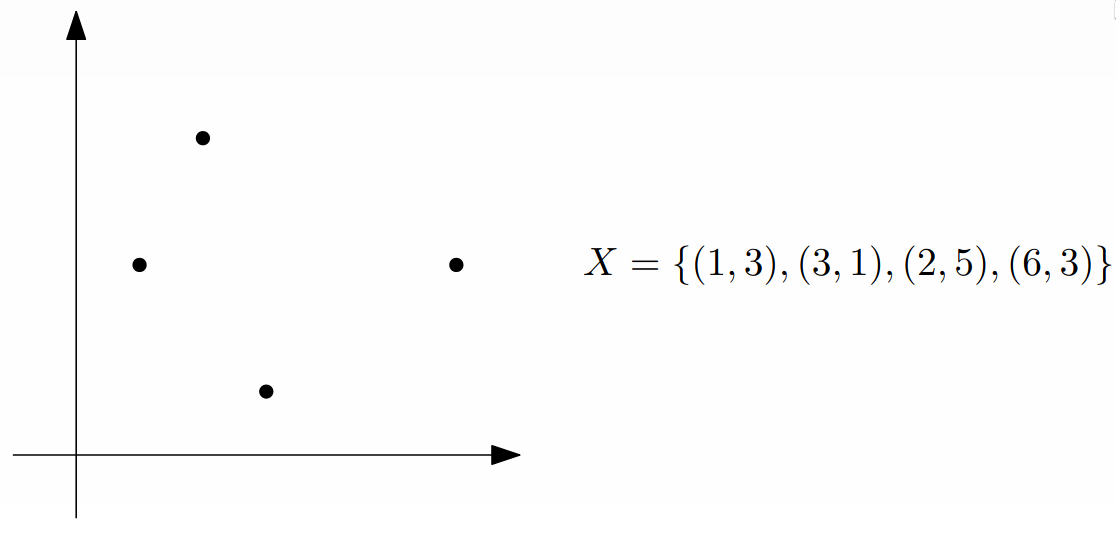
\includegraphics[width=0.5\textwidth]{img/2025-04-14-09-43-27.png}
\end{center}
E' il quadrilatero che ha i punti come vertici. Ha fatto un discorso con triangoli e piani, va beh viene questo:
\begin{center}
  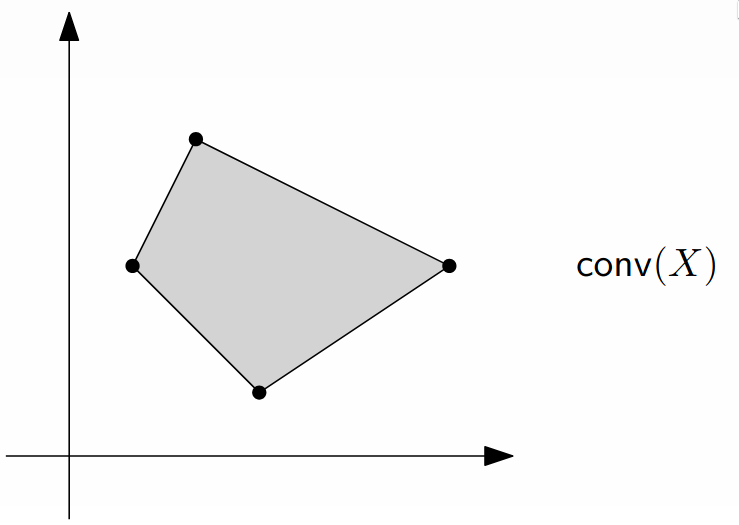
\includegraphics[width=0.5\textwidth]{img/2025-04-14-09-45-25.png}
\end{center}
}

\nt{
  E' possibile che un punto non faccia parte dei vertici, ma che sia un punto interno. Infatti, se nell'esempio di prima mettessimo un punto al centro, l'inviluppo convesso non cambierebbe.
}

\subsection{Coni Convessi}
Gli inviluppi convessi piu' semplici. TODO: definizione cono e cono convesso, con esempi

Il cono convesso si genera date le direzioni

\subsection{Teorema di Motzkin}
Operazione che codifica l'intuizione che i concetti di coni e inviluppi hanno a che fare con i poliedri. Il cono convesso cattura il concetto di possibile illimitatezza, quindi mescoliamo le due cose usando le somme fra insiemi di vettori.

\thm{Teorema di Motzkin}{
  $ P \subseteq \mathbb{R}^{n} $ e' un poliedro sse esistono $ X,V $ finiti tali che $ P = conv(X) + cono(V) $
}
La cosa cruciale e' il legame fra il mondo di vincoli e quello di punti e direzioni. Non lo dimostriamo perche no.

\nt{
  Sta roba puo' sembrare ovvia in 2d, ma in dimensioni piu' alte non e' cosi ovvio ed e' per questo che e' tanta roba.
}

\subsection{Due Rappresentazioni}
All'aumentare delle dimensioni, i vertici aumentano in modo esponenziale $ 2^{n} $, mentre i vincoli aumentano molto piu' lentamente $ 2n $. Male male sta cosa, perche' noi siamo INFORMATICI (anche Ugo), e ci servono algoritmi rapidi.

\subsection{Teorema Fondamentale}
\thm{}{
  Sia $ P = \{x | Ax \leq b\} $ e siano $ x_1,...,x_s, v_1,...,v_t \in \mathbb{R}^{n} $ tali che
  \[
    P = conv(\{x_1,...,x_s\}) + cono(\{v_1,...,v_t\})
  \]
  Allora il problema $ max \{cx | Ax \leq b\} $
}

\nt{
  La condizione $ cv_j \leq 0 $ significa che andando verso le direzioni, la funzione da massimizzare decresce. Dato che le soluzioni ammissibili possono essere illimitate solo lungo queste direzioni, significa che la funzione obbiettivo non puo' aumentare illimitatamente.
}

\pf{Dimostrazione}{
  
}

\section{Dualita'}
% \end{document}
